%%%%%%%%%%%%%%%%%%%%%%%%%%%%%%%%%%%%%%%%%%%%%%%%%%%%%%%%%%%%%%%%%%%%%%
% Source: http://www.howtotex.com
%%%%%%%%%%%%%%%%%%%%%%%%%%%%%%%%%%%%%%%%%%%%%%%%%%%%%%%%%%%%%%%%%%%%%%
\documentclass[paper=a4, fontsize=11pt]{scrartcl}
\usepackage[T1]{fontenc}
\usepackage{fourier}

%\usepackage{minted}
%\usemintedstyle{cpp}
%\usemintedstyle{trac}
%\newminted{cpp}{bgcolor=col, linenos=true}

\usepackage{xcolor}
\usepackage[pdftex]{graphicx}  
\usepackage[]{minted}
\setminted{linenos,bgcolor=col, obeytabs=true}
\definecolor{col}{rgb}{0.85,0.85,0.85}
%\BeforeBeginEnvironment{minted}{\begin{tcolorbox}}%
%\AfterEndEnvironment{minted}{\end{tcolorbox}}%

\usepackage[english]{babel}                                                                                                                     % English language/hyphenation
\usepackage[protrusion=true,expansion=true]{microtype}  
\usepackage{amsmath,amsfonts,amsthm} % Math packages
\newcommand*{\rttensor}[1]{\overline{\overline{#1}}}
\newcommand{\pfrac}[2]{\frac{\partial#1}{\partial#2}}



\usepackage{url}
\usepackage{hyperref}


\usepackage[numbers]{natbib}
%\usepackage[style=ieee]{biblatex}

%%% Custom sectioning

\usepackage{sectsty}
\allsectionsfont{\centering \normalfont\scshape}


%%% Custom headers/footers (fancyhdr package)
\usepackage{fancyhdr}
\pagestyle{fancyplain}    
\fancyhead{}% No page header
\fancyfoot[L]{}% Empty 
\fancyfoot[C]{}% Empty
\fancyfoot[R]{\thepage}% Pagenumbering
\renewcommand{\headrulewidth}{0pt}% Remove header underlines
\renewcommand{\footrulewidth}{0pt}% Remove footer underlines
\setlength{\headheight}{10.6pt}


%%% Equation and float numbering
\numberwithin{equation}{section}                % Equationnumbering: section.eq#
\numberwithin{figure}{section}                  % Figurenumbering: section.fig#
\numberwithin{table}{section}                           % Tablenumbering: section.tab#


%%% Maketitle metadata
\newcommand{\horrule}[1]{\rule{\linewidth}{#1}}         % Horizontal rule

\title{%\vspace{-1in}      
    \usefont{OT1}{bch}{b}{n}
    \normalfont\normalsize \textsc{Kevin T. Crofton Department of Aerospace and Ocean Engineering} \\ [25pt]
    \horrule{0.5pt} \\[0.4cm]
    \huge Magneto Rayleigh-Taylor Instability for an Annulus using Finite Volume Method with the MagnetoHydroDynamic Equations  \\
    \horrule{2pt} \\[0.5cm]}
\author{\normalfont\normalsize
  Robert Masti\\[-3pt]  
  \normalsize\today}
\date{}


%%% Begin document
\begin{document}
\maketitle
\section{MRT Overview \& Simulation Setup}\label{sec:ovrvw}
The magneto Rayleigh-Taylor instability (MRT) occurs when there is a heavy fluid supported by a light fluid under the influence of gravity with the addition of magnetic fields. Depending on the orientation of these magnetic fields they can have stabilizing characteristics for the growth of this instability. MRT is a hydrodynamic instability so it can be modeled using the ideal MagnetoHydroDynamic (MHD) equations. This instability is one of the most detrimental instabilities in the plasma communities attempt to reach fusion ignition. Specifically as it applies to inertial confinement fusion devices such as the one at NIF in the Direct Drive concept shown in Figure~\ref{fig:ovrvw:dd} part (c). The densities, pressures, and acceleration are going to be taken from \href{https://www.astro.princeton.edu/~jstone/Athena/tests/rt/rt.html}{Athena Webpage} to at least get the simulation setup, and then transition to realistic densities, pressures, and acceleration.


  \begin{figure}[!htb]
    \centering
    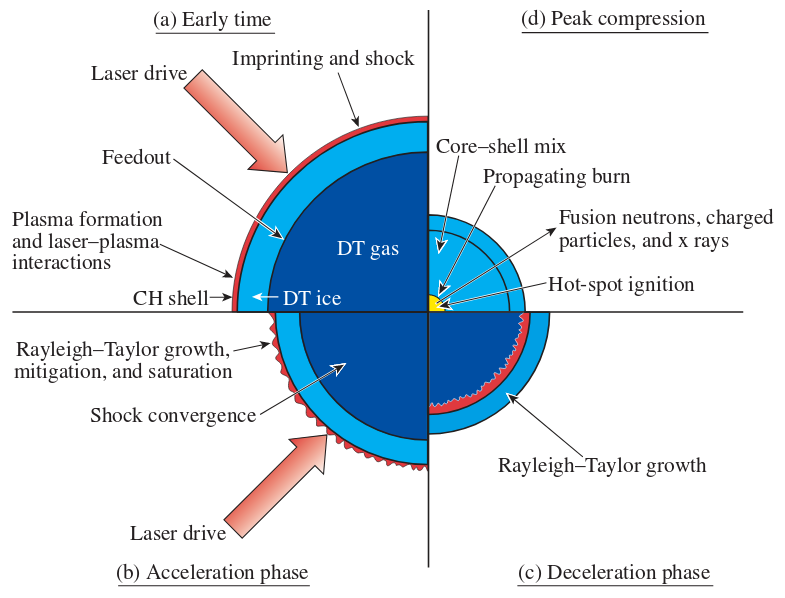
\includegraphics[width=0.9\linewidth]{fig/DDfusion}\label{fig:ovrvw:dd}
    \caption{Shows the four main stages during a typical direct-drive target implosion.\cite{craxton2015}}
  \end{figure}

\subsection{MHD Equation System}

The mhd equations allow for the incorporation of electric and magnetic fields as they influence a conducting medium. It has the continuity, conservation of momentum and energy like in Euler equation, but it has the addition of an induction equation for the magnetic field. For a plasma there is co existing electrons and ions, and in MHD the electron fluid equations are used to derive the electric field used in the induction equation, and the extent of this electric field can extend or retract the equation system. Initially just the lorentz force term will be used as the electric field contribution to the induction equation. Assuming ideal gas EOS the MHD equations are given by

\minipage{\textwidth}
  \minipage{0.48\textwidth}
  \begin{align*}
    \pfrac{\rho}{t} + \nabla \cdot \left[\rho \mathbf{u}\right] &= 0 \\
    \pfrac{\rho \mathbf{u}}{t} + \nabla \cdot \left[\rho \mathbf{u}\mathbf{u}^T - \mathbf{b}\mathbf{b}^T + \mathbb{I}\left(P + \frac{1}{2}|\mathbf{b}|^2\right)\right] &= 0 \\
    \pfrac{\epsilon}{t} + \nabla \cdot \left[\left(\epsilon + P + \frac{1}{2}|\mathbf{b}|^2\right)\mathbf{u}- \mathbf{b}\cdot\mathbf{u}\mathbf{b}\right] &= 0 \\
    \pfrac{\mathbf{b}}{t} + \nabla\times\mathbf{e} &= 0 \\
  \end{align*}
  \endminipage\hfill
  \minipage{0.48\textwidth}
  \begin{align*}
    \mathbf{b} &= \frac{\mathbf{B}}{\sqrt{\mu_0}} \\
    \mathbf{e} &= - \mathbf{u} \times \mathbf{b} +\left(\mathbf{e}^{external}\rightarrow\mathbf{0}\right)\\
    \epsilon &= \epsilon_{internal} + \frac{1}{2}\rho|\mathbf{u}|^2 + \frac{1}{2}|\mathbf{b}|^2\\
    P &=\rho \epsilon_{internal} (\gamma - 1) \\
  \end{align*}
  \endminipage\hfill
  \endminipage, where there is no external electric fields ($e.q.\;\eta \mathbf{j}$). The equation for the magnetic field must be manipulated with vector identities into a divergence form through
  \begin{align*}
    \pfrac{\mathbf{b}}{t} + \nabla\times(-\mathbf{u}\times\mathbf{b}) &= 0\\
    \pfrac{\mathbf{b}}{t} - \left[\mathbf{u}(\nabla\cdot\mathbf{b})-\mathbf{b}(\nabla\cdot\mathbf{u})+(\mathbf{b}\cdot \nabla)\mathbf{u}-(\mathbf{u}\cdot\nabla)\mathbf{b}\right] &= 0\\
    \pfrac{\mathbf{b}}{t} - \left[\nabla\cdot(\mathbf{b}\mathbf{u}^T)-\nabla\cdot(\mathbf{u}\mathbf{b}^T)\right] &= 0\\
    \pfrac{\mathbf{b}}{t} + \nabla\cdot\left[\mathbf{u}\mathbf{b}^T-\mathbf{b}\mathbf{u}^T\right] &= 0\\
  \end{align*}, and it now is in divergence form which can be used to write into the tensor product form. The conservative variable are density, momentum, total energy density, and magnetic field. For the given problem however it is more convenient to rewrite as
\begin{equation}\label{eqn:mhdvector}
  \pfrac{\mathbf{Q}}{t} + \nabla \cdot \rttensor{T} = 0
\end{equation}
where $\mathbf{Q}$ is the conserved variables vector, and $\rttensor{T}$ is the flux tensor. Where the conserved variables vector, and flux tensor, are given by
\[
  \mathbf{Q}=
  \begin{bmatrix}
    \rho  \\
    \rho \mathbf{u}  \\
    \epsilon\\
    \mathbf{b} 
  \end{bmatrix}
  ,\quad \rttensor{T} =
  \begin{bmatrix}
    \rho \mathbf{u}  \\
    \rho \mathbf{u}\mathbf{u}^T - \mathbf{b}\mathbf{b}^T + \mathbb{I}\left(P + \frac{1}{2}|\mathbf{b}|^2\right)\\
    \left(\epsilon + P + \frac{1}{2}|\mathbf{b}|^2\right)\mathbf{u}- \mathbf{b}\cdot\mathbf{u}\mathbf{b}\\
    \mathbf{u}\mathbf{b}^T-\mathbf{b}\mathbf{u}^T
  \end{bmatrix}
\]
, respectively. 

\subsection{Discretization \& Flux Formulation}
  \begin{figure}[!htb]
    \centering
    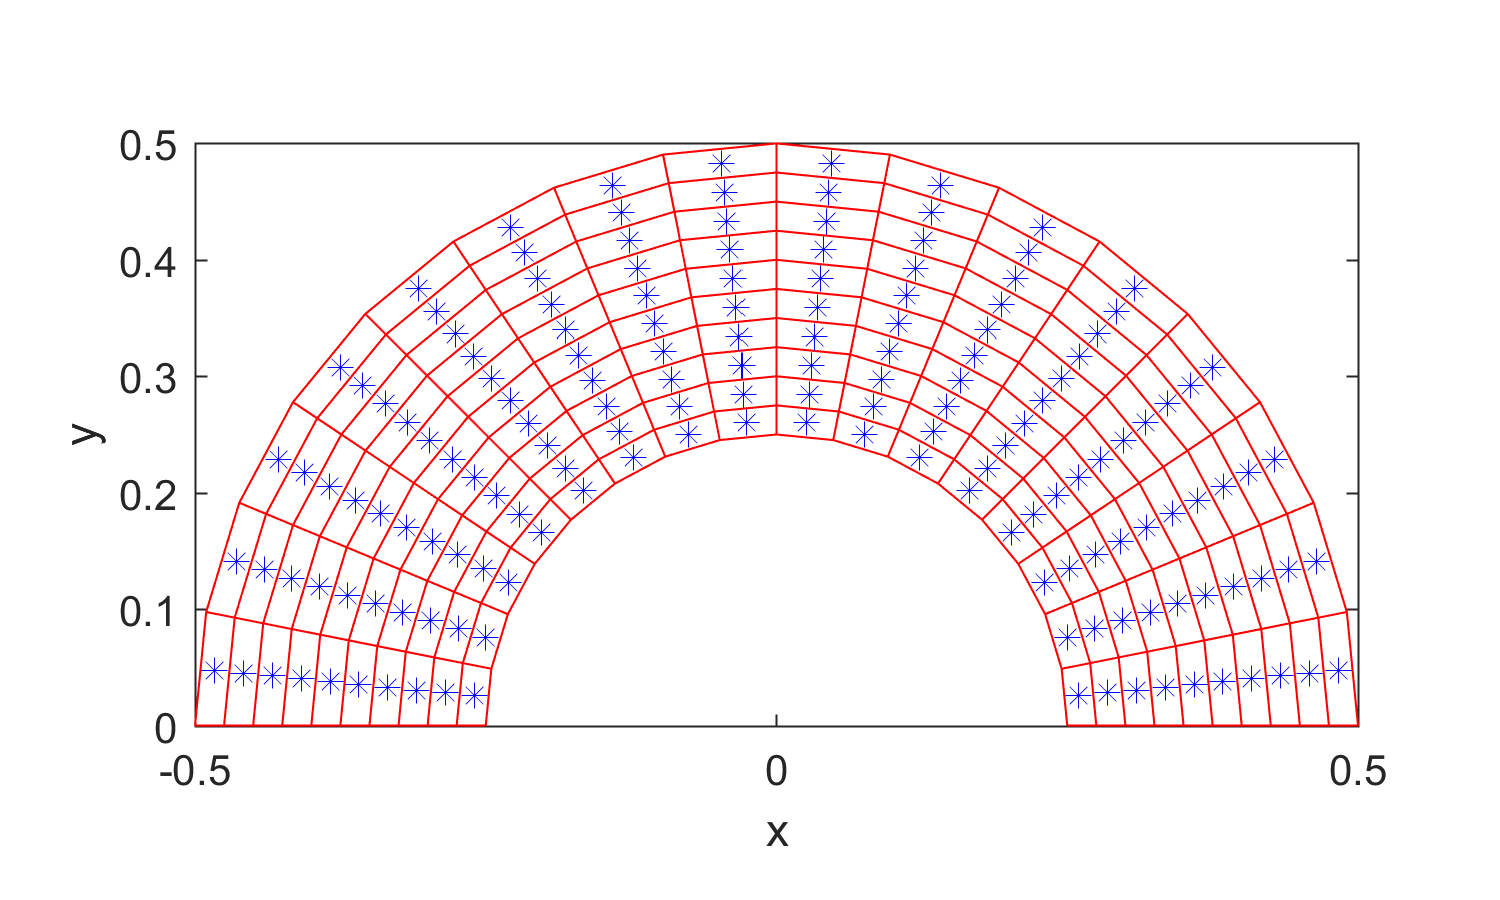
\includegraphics[width=1.0\linewidth]{fig/16x10mesh}\label{fig:ovrvw:mesh}
    \caption{A mesh example using 16 cells in the i direction and 10 cells in the j direction with cell centers highlighted using 4 partitions}
  \end{figure}

The simulation setup will use a discretization shown in Figure~\ref{fig:ovrvw:mesh} where the coordinates are unitless currently. The mesh generation is done in matlab for this simplistic geometry. In order to evaluate the flux in the x and y direction the normal vectors on the cell faces are required. With the normal vectors and areas known the fluxes can be determined for MHD in curvilinear coordinates as

\begin{equation} \label{eqn:mhdvecflux}
  \pfrac{\mathbf{Q}}{t} + \pfrac{\mathbf{F}}{x} + \pfrac{\mathbf{G}}{y} = 0
\end{equation},
where $\mathbf{F}$ is the $\hat{x}$ direction flux, and $\mathbf{G}$ is the $\hat{y}$ direction flux. Expanding the flux tensor through evaluating the dyadic terms, and collecting non-zero unit vectors $\mathbf{F}$, and $\mathbf{G}$ can be easily found. Equation~\ref{eqn:mhdvecflux} can be expanded into for cartesian coordinates into

\[
  \pfrac{}{t}
  \begin{bmatrix}
    \rho  \\
    \rho u  \\
    \rho v \\
    \rho w \\
    \epsilon\\
    b_x \\
    b_y \\
    b_z 
  \end{bmatrix}
  \;+\;\pfrac{}{x}
  \begin{bmatrix}
    \rho u  \\
    \rho u^2 + P + \frac{1}{2}|\mathbf{b}|^2 - b_x^2\\
    \rho u v - b_x b_y \\
    \rho u w - b_x b_z \\
    \left(\epsilon+ P + \frac{1}{2}|\mathbf{b}|^2 \right) u - b_x \mathbf{u}\cdot\mathbf{b}\\
    0 \\
    b_y u - b_x v \\
    b_z u - b_x w 
  \end{bmatrix}
  \;+\;\pfrac{}{y}
  \begin{bmatrix}
    \rho v  \\
    \rho v u - b_y b_x\\
    \rho v^2 + P + \frac{1}{2}|\mathbf{b}|^2 - b_y^2\\
    \rho v w - b_y b_z \\
    \left(\epsilon+ P + \frac{1}{2}|\mathbf{b}|^2  \right) v - b_y\mathbf{u}\cdot\mathbf{b}\\
    b_x v - b_y u \\
    0 \\
    b_z v - b_y w 
  \end{bmatrix}
  =0
\]

For an arbitrarily oriented cell with interface normal $\hat{n} = n_x \hat{x} + n_y\hat{y}$ that maps to compuational grid $(i,j)\rightarrow(\eta,\xi)$) this form can be rewritten as

\[
  \pfrac{}{t}
  \begin{bmatrix}
    \rho  \\
    \rho u  \\
    \rho v \\
    \rho w \\
    \epsilon\\
    b_x \\
    b_y \\
    b_z 
  \end{bmatrix}
  \;+\;\pfrac{}{\eta}
  \begin{bmatrix}
    \rho c_*  \\
    \rho u c_* + P n_x + \frac{1}{2}|\mathbf{b}|^2 n_x- b_x b_*\\
    \rho v c_* + P n_y + \frac{1}{2}|\mathbf{b}|^2 n_y - b_y b_* \\
    \rho w c_* - b_z b_*\\
    \left(\epsilon+ P + \frac{1}{2}|\mathbf{b}|^2 \right) c_* - b_* \mathbf{u}\cdot\mathbf{b}\\
    b_x c_* - b_* u\\
    b_y c_* - b_* v \\
    b_z c_* - b_* w 
  \end{bmatrix}
  \;+\;\pfrac{}{\xi}
  \begin{bmatrix}
    \rho c_*  \\
    \rho u c_* + P n_x + \frac{1}{2}|\mathbf{b}|^2 n_x - b_x b_* \\
    \rho v c_* + P n_y + \frac{1}{2}|\mathbf{b}|^2 n_y - b_y b_* \\
    \rho w c_* - b_z b_* \\
    \left(\epsilon+ P + \frac{1}{2}|\mathbf{b}|^2  \right) c_* - b_*\mathbf{u}\cdot\mathbf{b}\\
    b_x c_* - b_* u \\
    b_y c_* - b_* v \\
    b_z c_* - b_* w 
  \end{bmatrix}
  =0
\]
where $c_* = u n_x + v n_y$, and $b_* = b_x n_x + b_y n_y $, which results in the new form
\begin{equation} \label{eqn:mhdvecfluxarb}
  \pfrac{\mathbf{Q}}{t} + \pfrac{\mathbf{F}_\eta}{\eta} + \pfrac{\mathbf{G}_\xi}{\xi} = 0
\end{equation}.

\section{The Code}\label{sec:code}
The code is using Finite Volume Method (FVM) with Monotone Upwinding Scheme for Conservation Law for the reconstruction of cell averaged values to interface states. Second order reconstruction is used along with a three wave flux Approximate Riemann Solver (ARS). Eventually an eight wave form will be implemented, but for now use HLL flux \cite{harten1983}

\subsection{Mesh Read}

The first mpi capable modification to the serial code is the mesh reader in which rank 0 will read in the mesh and distribute to all of the other siblings. Note to try and keep as much of the serial code the same Eigen row major matrices are used to fill throughout as it makes the implementation cleaner. Mesh block has the following inputs and outputs

\begin{minted}{cpp}
MPI_Comm meshBlock(
    const string mesh,            //In: mesh name to read
    const string outputFolder,    //In: name of output dir
    RowMajorMatrixXd &xcLg,       //Out: local x center coord
    RowMajorMatrixXd &ycLg,       //Out: local y center coord
    RowMajorMatrixXd &nixL,       //Out: local x comp norm vec i dir
    RowMajorMatrixXd &niyL,       //Out: local y comp norm vec i dir
    RowMajorMatrixXd &njxL,       //Out: local x comp norm vec j dir
    RowMajorMatrixXd &njyL,       //Out: local y comp norm vec j dir
    RowMajorMatrixXd &AiL,        //Out: local area i dir
    RowMajorMatrixXd &AjL,        //Out: local area j dir
    RowMajorMatrixXd &VolumeL,    //Out: local cell volume
    const constants C)                  
\end{minted}

\textbf{meshBlock} takes in the mesh filename writes out the geometry, and distributes \& fills all the local geometry needed to run the FVM. It also returns a new MPI communicator in which it has special features in which it knows the nearest neighbor partitions. First find the number of partition to use in the x and y using squares

\begin{figure}[!htb]
  \centering
  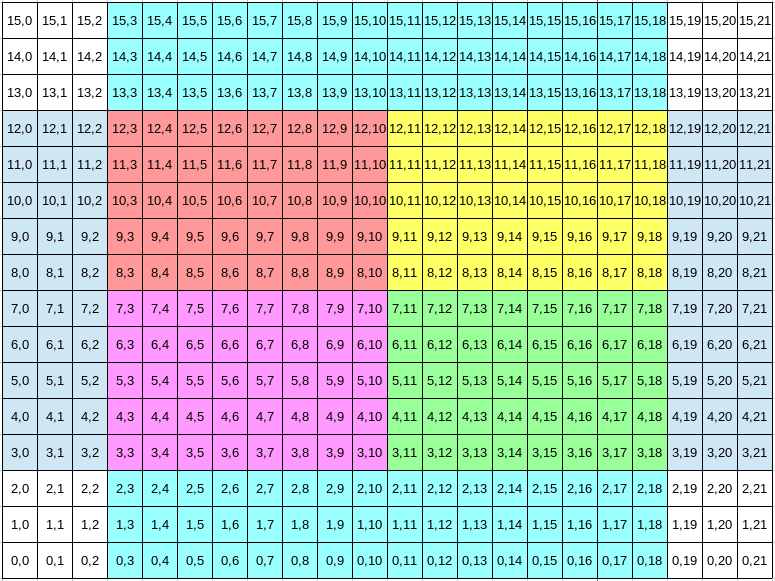
\includegraphics[width=1.0\linewidth]{fig/16x10compDomain}\label{fig:code:compDom}
  \caption{Representation of figure~\ref{fig:ovrvw:mesh} in the computational domain with its extrapolated ghost cells (number of layers = 3) partitioned into 4 as an example.}
\end{figure}

\begin{figure}[!htb]
  \centering
  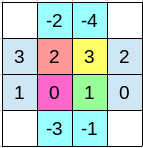
\includegraphics[width=0.175\linewidth]{fig/partition}\label{fig:code:part}
  \caption{MPI\_Cart cartesian communicator setup for 4 partitions referencing the physical, and computational grid in figures~\ref{fig:ovrvw:mesh}, and~\ref{fig:code:compDom}, respectively.}
\end{figure}



\begin{minted}{cpp}
  MPI_Comm_size(MPI_COMM_WORLD, &size)
  int cnt = size;
  int n = 0;
  while (cnt >= 2){
    cnt = cnt/2;
    n++;
  }
  nj = pow(2, (n/2)); // partitions in the vert direction
  ni = pow(2, (n/2)+n%2); // partitions in the horiz direction
\end{minted}

Currently the number of partitions requested has to be a power of 2, but will be revisited. With the number of partitions in the i and j known the new communicator can be created through

\begin{minted}{cpp}
  int dim[2] = {nj, ni};        // 2 int array for MPI_Cart_Create
  int reorder = FALSE;          // Reorder for fastest comm
  int period[2] = {FALSE, TRUE};// periodic boundary partit

  MPI_Comm com2d; // Setup cartesian communicator
  MPI_Cart_create(MPI_COMM_WORLD, 2, dim, period, reorder, &com2d);
  MPI_Comm_rank(com2d, &rank);
\end{minted}
, where \href{https://www.mpich.org/static/docs/v3.2/www3/MPI\_Cart\_create.html}{MPI\_Cart\_Create} creates a grid of the partitions with periodic capabilities. With the number of partitions in i and j set rank 0 fetches the data from the mesh file currently created using matlab. With the coordinates that define the cell known the ghost cell coordinates are extrapolated from the interior, and the areas, normal vectors, and volumes of the cells are then computed which looks like
\begin{minted}{cpp}
if(rank == 0){
  RowMajorMatrixXd xn, yn;
  RowMajorMatrixXd xc, yc;
  inputMesh(xn, yn, xc, yc, mesh);
  ...
  extrapCopyCoords(xc_g, yc_g, xc, yc, C);
  ...
  computeArea(Ai, Aj, xn, yn);
  computeNormalVectors(nix, niy, njx, njy, xn, yn, Ai, Aj);
  computeVolume(Volume, xn, yn);
\end{minted}
. Note that rank 0 computes these quantities globally for the entire domain like in figure~\ref{fig:code:compDom} into the RowMatrixXd class which is defined as
\begin{minted}{cpp}
typedef Matrix<double,Dynamic,Dynamic,RowMajor> RowMajorMatrixXd;
\end{minted}
, where using this row major format allows for easy incorporation with MPICH. With all global geometry defined it is then sent to the other ranks by first sending the size it expects to receive in $nb$

\begin{minted}{cpp}
  int nx = xc.cols();
  int ny = xc.rows(); 
  int nxb = nx/ni; // nx per partition
  int nyb = ny/nj; // ny per partition
  
  nb[0] = nxb;
  nb[1] = nyb;
  for(int r = 1; r < size; r++)
    MPI_Send(nb, 2, MPI_INT, r, 999, com2d);
\end{minted}
, and then the arrays can be sent using the eigen block command 
\begin{minted}{cpp}
// loop over all ranks
for(int j = 0; j < nj; j++){
  for(int i = 0; i < ni; i++){
    int r = j*ni+i; // current rank
    if (r >= 1){ // mpi send
      //block(row start, col start, rows, cols)
      temp = xcg.block(nyb*j, nxb*i, nybg, nxbg); 
      MPI_Send(temp.data(), nxbg*nybg, MPI_DOUBLE, r, 111, com2d);
      ...
    }
    else{ // rank 0 fills its own local geo
      xcLg = xcg.block(nyb*j, nxb*i, nybg, nxbg);
      ...
    } 
\end{minted}
. All the data then has been sent from rank 0 and now is received through

\begin{minted}{cpp}
if(rank == 0){
  ...
}
else{
  int source = 0;
  MPI_Status status;
  // receive sizes
  MPI_Recv(&nb, 2, MPI_INT, source, 999, com2d, &status); 
  ...
  // receive directly into eigen array
  MPI_Recv(xcLg.data(), nxbg*nybg, MPI_DOUBLE, source, 111, com2d, 
    &status);
  ...
}
\end{minted}
. With all the geometry locally defined the only other mpi function needed is for halo exchange/boundary conditions. 

\subsection{Halo Exchange \& Boundary Conditions}
Every partition for this code must send its ghost cell layer $\mathbf{Q}$'s to its neighboring partitions unless it is a physical boundary. Periodic physical boundaries are used for the left and right walls, while a perfectly conducting wall is used for the top and bottom walls. The function that does these operations is
\begin{minted}{cpp}
void mpiSetBc(
    Map2Eigen* U,                 //Out: conserved vars
    const RowMajorMatrixXd& nix,  //In: norm vec xcomp i dir
    const RowMajorMatrixXd& niy,  //In: norm vec ycomp i dir
    const RowMajorMatrixXd& njx,  //In: norm vec xcomp j dir
    const RowMajorMatrixXd& njy,  //In: norm vec ycomp j dir
    MPI_Comm& com2d,              //In: Communicator 
    constants C)                   
{
\end{minted}
. Note Map2Eigen is a wrapper that sets up a 3 dimensional array that is mapped to a single C array set up in row major format like
\begin{minted}{cpp}
U->Q_raw = {rho, u, v, w, p, bx, by, bz, rho, u, v, ...}
U->Q[rho](j, i)
U->Q[u](j, i)
U->Q[v](j, i)
\end{minted}
. Using this map allows for the structure of the serial code to not be altered while being MPI compatible. With the cartesian MPI communicator nearest neighboring partitions are found using \href{https://www.mpich.org/static/docs/v3.2/www3/MPI_Cart_shift.html}{MPI\_Cart\_Shift} of which internally keeps track of physical walls ($-$ number), and periodic walls
\begin{minted}{cpp}
int r, l, u, d;
int rank;
MPI_Comm_rank(com2d, &rank);
//MPI_Cart_Shift(communicator, direction, displacement, source, dest)
MPI_Cart_shift(com2d, 0, 1, &d, &u); 
MPI_Cart_shift(com2d, 1, 1, &l, &r);
\end{minted}
. Applying as an example partition 3 in figure~\ref{fig:code:part} will have left $=$ 2, right $=$ 2, down $=$ 1, and up $=$ -4. With the nearest neighbors of every partition known apply boundary conditions/halo exchange for all boundaries. The left and right boundaries are periodic (with the exception of x and y component quantities of $\mathbf{Q}$), and to send the data 
\begin{minted}{cpp}
int sendSize = njc*C.num_ghost*NEQ; // njc number of rows with ghost
Map2Eigen *tempLout = new Map2Eigen(njc , C.num_ghost, NEQ);
int ic = C.num_ghost;
int sign = +1;
int out = l;
int tag = 222; // right recv
for(int i = 0; i < C.num_ghost; i++)
  for(int eq = 0; eq < NEQ; eq++)
    tempLout->Q[eq].col(i) = U->Q[eq].col(ic+sign*i);
if(l>rank){
  // flip sign for phys periodic boundary
  tempLout->Q[uid]  =-1.0*tempLout->Q[uid];
  tempLout->Q[vid]  =-1.0*tempLout->Q[vid];
  tempLout->Q[bxid] =-1.0*tempLout->Q[bxid];
  tempLout->Q[byid] =-1.0*tempLout->Q[byid];
}
// sent to left 
MPI_Isend(tempLout->Q_raw, sendSize, MPI_DOUBLE, out, tag, 
  com2d, &requestOut[0]);//tag222 is right
\end{minted}
for the left which can similarly be done for the right. The upper and lower surface physical boundary is a perfectly conducting wall so that the normal component of $\mathbf{u}$, and $\mathbf{b}$, is $0$ at the wall, and with normal vector is given by
\begin{align*}
  u_g &= -n_x(u n_x + v n_y) - n_y(-u n_y + v n_x)\\
  v_g &= -n_y(u n_x + v n_y) + n_x(-u n_y + v n_x)\\
  b_{xg} &= -n_x(b_x n_x+b_y n_y) - n_y( -b_x n_y + b_y n_x)\\
  b_{yg} &= -n_y(b_x n_x + b_y n_y) + n_x(-b_x n_y + b_y n_x)
\end{align*}
, where $u,v,b_x,b_y$ are the interior cell values. The other quantities in $\mathbf{Q}$ ($\rho, \rho w, \epsilon, b_z$) are extrapolated from the interior


\clearpage
 \bibliographystyle{IEEEtran}
  \bibliography{reference}
%%% End document
\end{document}
